\chapter[SCP-001 螺旋路]{
	SCP-001 Dr. Mann - The Spiral Path \\
	SCP-001 螺旋路
}

\label{chap:SCP-001.the.spiral.path}

\begin{figure}[H]
	\centering
	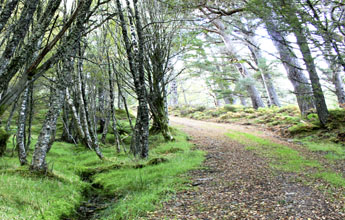
\includegraphics[width=0.5\linewidth]{images/SCP.001.the.spiral.path.jpg}
	\caption*{SCP-001的一部分}
\end{figure}

\bb{项目编号:}SCP-001

\bb{项目等级:}Embla

\bb{特殊收容程序:}SCP-001于[已编辑]州,Site 0就地收容。一道围篱沿著SCP-001的可观察半径筑起。为了安全起见,Site 0随时都需布署五名或以上的武装守卫以防止未经授权的进入。邻近的物理实验室也需随时运作以研究任何异常。

一块刻有提醒标语的金属告示牌应随时维护以保持在最佳状态。任何损伤都需立即回报以进行修补。

\bb{描述:}SCP-001是一条位于林中的环状砾石小径。以逆时针方向行走时,路途会是持续的上坡,就算通过起始点亦然;以顺时针方向行走时,路途的上、下坡数量是相同的,而没有异常。

存取SCP-001的实验记录需五级授权。

监督者议会(Overseer Council)的新成员需阅读\hyperref[sec:DOC-001-05]{文档001-O5}。

\chapter{文档001-O5}

\label{chap:DOC-001-05}

如果你正在阅读这行字的话,那恭喜你。我们的其中一员离世了。某种东西杀死了我们的一份子。或许是只怪物,或是来自GOC的对手。或是我们玩火自焚,像Aaron那样。当然,不会是因为年龄。我们在那方面保持的很好,是不?无论如何,一位看守逝去了。或许是Jason,或许是Agnes,或许是我。老天,我如果不是下一个死的,我会很惊讶。我永远都是那个最操劳的。

我写这些东西的时候,是把你当成一个人类来看待,这会是你此生最后一次受到礼遇,所以我希望你会感激。

无论你是谁,无论你以前做过什么,你被拉进这里之前一定达到了很高的层级。你一定会发现事情有些蹊跷,不是那么单纯。我不知道你已经听过了多少,或你自己拼凑出多少。整件事的关键在于:SCP的回收与取得若不是演出来的,就是凭空捏造的。整个基金会历史上根本没有「回收」过任何的SCP。

我应该从头开始。让我来说个故事。

Aaron Siegel是一名1891年在康乃尔大学进行研究的物理学家。他天赋异秉,如果没有踏上这条路的话,我想他的名字会与爱迪生、爱因斯坦跟霍金齐名。我与他非常熟稔。他曾经是,以后大概也会是,我的兄长。同时,他也是一位热忱的业馀博物学家,喜欢在森林中健行。有一天,当他正要拜访我们位于Essex乡间的老家时,他遇到一条砾石小径。他决定沿着小径走一段路,并且注意到这条路不断往上延伸,远超过它应有的长度。他本该能走到附近的山丘上。但他发现自己回到原本走入的地方,而没有往下的路程。如果是另一个人,就会假设是自己感官出了问题然后离去。但,Aaron是一个顽固的人。他深入调查。他发现这条小径不遵守欧几里德的纯粹几何学。就像他之前的Saccheri\footnote{\bb{译注:}Giovanni Girolamo Saccheri(1667-1733),意大利耶稣会修士、经院哲学家与数学家,是非欧几何的先驱者之一。}一样,他找到了某种与直线性质相违的异数。

于是他研究起这条路径。所衍生出的方程式构成了你所拿到的资料的其中一部分。你总有一天会真正理解这些文字的意义。他在附近盖了一间小屋作为临时的实验室。他的第一次实验制造了一把可以打开所有门锁的钥匙,现在被以SCP-005的名字收容着。

他找了其他人加入。我身为他的兄弟,自然是他首先联系的人。我那时在哈佛学医。刚开始我以为他疯了,但当他向我展示小径及钥匙的时候,我知道我必须从这里面学到更多。与我们共事的还有几个朋友与同事。他们大多都已经逝去……但,我们是一切的核心,基金会围绕着我们而建立起来。

刚开始,我们专注于新的发现,专注于我们能做到的事情。我们有着很高的期待与抱负。我们觉得自己能改变世界、拯救众生。我们希望能喂养、庇护、医治所有的人。Thomas Carter\footnote{\bb{译注:}疑为Thomas Henry Carter(1854-1911),美国参议员。}资助我们,我们之中没有一个是穷人,但是还是钱马上就用光了。Thomas利用他跟华尔街及华盛顿的关系帮我们筹措经费。他向金主们展示了我们的一点成果,并对天发誓只会用在正途上;我兄长的未婚妻Agnes Peterson是一位懂得如何建立组织的人。我们其他人根本不晓得怎么经营一个像样的团体。是她整饬了这些梦想家与狂人,把一盘散沙、只会东奔西跑的我们组合成一个团体。

很快地,我们建立起第一个机构。但仍然保持神秘。当我们想大声宣告自己的发现时,我们也同时害怕它们会被夺走。我们告诉自己,这都只是暂时的,等我们打好基础,一定会昭告世人。我们刚开始很小心。只制造一些小而安全,甚至很有用的道具。像不老泉、弹力球、内战雕像。随着我们的信心渐增,我们开始在人类身上实验。像混凝土人就是自愿的。或是肚子里有个行星的男人,原本只是个流浪汉,但我们让他有了特点,不是吗?

太容易了,或许从一条小小的泥巴路能找到这么多东西看来可笑,但这些发现就只是一个接着一个,不断流泄而出。这简直就像是有什么东西在背后帮助我们一样。

但接下来,事情开始脱序。Aaron在玩弄他的方程式时,意外衍生出丢失的数字。我在实验室里,发现自己制造了僵尸瘟疫。但我们对自己的计画太过投入,更多的研究带来了梦魇管线还有楼梯井。我们才知道应该找人帮忙了。Thomas对军方展示了我们的成果。告诉他们这些东西是我们「找到」、「发现」的。我们胡诌了几个名字像「普罗米修斯实验室」和「混沌分裂者」。他们就以个人名义掏出大把钞票。我们茁壮起来,并且向外扩张。我们在其他国家重复这样的生意。有些人买帐,有些人不,这样已经足够了。我们成为一个国际性的组织,招募更多的研究者,但很少有人怀疑自己的实验对象是来自我们的手中。有时候我们会安排某个项目被外勤人员「找到」,有时我们干脆直接写下报告。一张张的文件和一次次的收容失效。如果我们说一件事情如何如何,它就会是那样,直到永远。

当然,问题还是不断产生。Jeremy跟Thomas偷走了我们的实验成果,来成立他们荒谬的俱乐部。我们的一个研究员发起疯来,开始崇拜机器,并带着足以成为威胁的知识逃走了。我们至今仍在处理这些小组织造成的影响。

我们遏制它们、掌握它们。我们欲罢不能,你懂吗?我们非但没有警觉,反而更加大胆。我把一个小男孩剖开,把他变成了一团憎恨的血肉。

理由,总是有理由。比如二三一,我们创造了她与她的姊妹。我们从孤儿院找到它们,并写好了剧本。没有意外,我们明白自己在做什么。这件事曾经有个理由,但如果我能想起来的话,肯定会遭天谴。我们之中没有一个人知道我的兄长在哪,或他成了什么东西。

我们继续前行。经过亚伯、经过血池、经过那该死的大蜥蜴,我们依旧前行。我们还能做什么?从这场由我们自己发动的灾难中幸存的唯一希望,就是深入了解它。骑虎难下也不足以形容我们的情况。但这不是我们真正担心的,也不应该是你所担心的,毕竟我们已经立足有数百年之久了。

真正让我挂心的是那些不是由我们所创造的异常。不,我这是头一回说实话。这些东西都不是从外面回收的。但其中一些,却不是我们的成果。它们就是……某一天出现了。它们被收容着,它们一直都被收容著。你还不懂吗?事情不再由我们掌控,从头到尾都不是。

